% ============================================================
% Figure 4: Graph-Based Clustering Pipeline
% ============================================================
\documentclass[border=5pt]{standalone}
\usepackage[T1]{fontenc}
\usepackage{tikz}
\usetikzlibrary{arrows.meta, positioning, shapes.geometric, fit, calc, chains}

\definecolor{cb1}{RGB}{0,101,189}
\definecolor{cb3}{RGB}{0,128,0}
\definecolor{cb4}{RGB}{230,159,0}
\definecolor{cbg}{RGB}{245,245,245}

\begin{document}
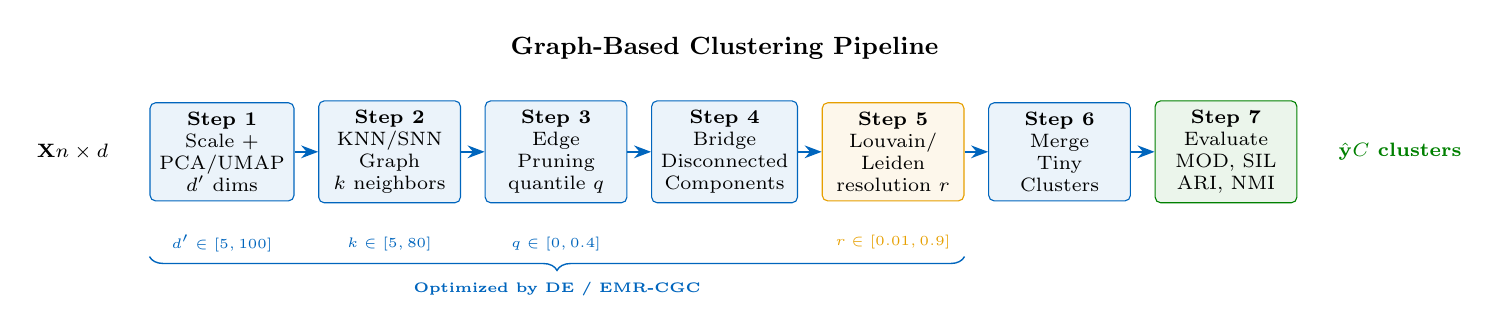
\begin{tikzpicture}[
    >=Stealth,
    font=\scriptsize,
    start chain=going right,
    node distance=0.3cm,
    pipe/.style={rectangle, rounded corners=2pt, draw=cb1, fill=cb1!8,
        minimum width=1.8cm, minimum height=1.2cm, align=center,
        font=\scriptsize, on chain},
    arr/.style={-Stealth, line width=0.7pt, cb1},
]

% Pipeline steps
\node[pipe] (s1) {\textbf{Step 1}\\Scale +\\PCA/UMAP\\$d' $ dims};
\node[pipe] (s2) {\textbf{Step 2}\\KNN/SNN\\Graph\\$k$ neighbors};
\node[pipe] (s3) {\textbf{Step 3}\\Edge\\Pruning\\quantile $q$};
\node[pipe] (s4) {\textbf{Step 4}\\Bridge\\Disconnected\\Components};
\node[pipe, draw=cb4, fill=cb4!8] (s5) {\textbf{Step 5}\\Louvain/\\Leiden\\resolution $r$};
\node[pipe] (s6) {\textbf{Step 6}\\Merge\\Tiny\\Clusters};
\node[pipe, draw=cb3, fill=cb3!8] (s7) {\textbf{Step 7}\\Evaluate\\MOD, SIL\\ARI, NMI};

% Arrows
\draw[arr] (s1) -- (s2);
\draw[arr] (s2) -- (s3);
\draw[arr] (s3) -- (s4);
\draw[arr] (s4) -- (s5);
\draw[arr] (s5) -- (s6);
\draw[arr] (s6) -- (s7);

% Input/Output
\node[left=0.4cm of s1, font=\scriptsize\bfseries] {$\mathbf{X}$\\$n \times d$};
\node[right=0.4cm of s7, font=\scriptsize\bfseries, cb3] {$\hat{\mathbf{y}}$\\$C$ clusters};

% Parameter annotations
\node[below=0.3cm of s1, font=\tiny\itshape, cb1] {$d' \in [5,100]$};
\node[below=0.3cm of s2, font=\tiny\itshape, cb1] {$k \in [5,80]$};
\node[below=0.3cm of s3, font=\tiny\itshape, cb1] {$q \in [0,0.4]$};
\node[below=0.3cm of s5, font=\tiny\itshape, cb4] {$r \in [0.01,0.9]$};

% Title
\node[above=0.4cm of s4, font=\small\bfseries] {Graph-Based Clustering Pipeline};

% Optimized by DE annotation
\draw[decorate, decoration={brace, amplitude=5pt, mirror}, cb1, line width=0.5pt]
    ([yshift=-0.7cm]s1.south west) -- ([yshift=-0.7cm]s5.south east)
    node[midway, below=0.2cm, font=\tiny\bfseries, cb1] {Optimized by DE / EMR-CGC};

\end{tikzpicture}
\end{document}
